% determine the decision rule

\section{Determine the decision rule under MENP Framework}
In the context of spectrum sensing, the lookup table $T_1$ can be pre-computed and stored in the detector before the detector is deployed. Once the probability of false alarm constraint(s) is(are) changed, the detector utilizes $T_1$ to get the MENP decision  rule parameters accordingly. The size of $T_1$ depends on the value of $M$, the range and the step of $k_i$.  Assume the value of $k_i$ ranges from $0$ to $\Gamma$ with step $\tau_0$, as $T_1$ is an exhaustive lookup table on the grid of $k_1, ..., k_M$, it has $(\frac{\Gamma}{\tau_0})^M$ items. Since a linear increase of $M$ leads to an exponential increase in the size of $T_1$, this method is no plausible for for the situation where $M$ is large. 

In \cite{zhang1999design, zhang2000efficient} Qian proposed an algorithm to solve this issue.  The algorithm can iteratively refine $k_i$ ($i=1, ..., M$) and generates an ENP test  such that among all ENP test with non-negative parameters it achieves the largest $P_d$ while keeping $P_{f_i}$ below the prescribed constraints. 
Obviously if the theoretical solution for \eqref{equ: problemstate} is an ENP test with positive parameters, this algorithm can acquire the optimal solution. 
In previous section, we showed the theatrical solution for \eqref{equ: problemstate} can be acquired by an ENP decision rule with positive parameters if $f_0(x) \neq 0$ a.e. on its domain. 
Hence the decision rule generated by \cite{zhang1999design, zhang2000efficient} is the optimal decision rule for \eqref{equ: problemstate} when $f_0(x) \neq 0$ holds a.e. on its domain.

The algorithm is summarized as follows. Let $t = \sum_{i=1}^{M}k_i$ and $\omega_i = \frac{k_i}{t}$ ($i=1, 2, ..., M$). In the algorithm, $\bom$ is termed the weight of the decision rule and $t$ is termed the threshold of the decision rule. Since only non-negative $k_i$ are considered, both $\omega_i, t$ are greater or equal to zero. The ENP test can be written in form of 
\begin{equation}
\label{qian dec}
f_0(x) \substack{H_0 \\ \geq \\ < \\ \bar{H}_0} t\sum_{i=1}^{M}\omega_if_i(x)\,.
\end{equation}

%Let $P_d$ and $\mathbf{P}_f$ denote the probability of detection and probability of false alarm of decision rule \eqref{qian dec} respectively. 
\cite{zhang2000efficient} illustrates that with $\omega_i$ ($i=1, 2, ..., M$) fixed, the probability of detection ($P_d$) and probability of false alarm ($\mathbf{P}_f$) under decision rule \eqref{qian dec} are continuous decreasing function with respect to $t$. 
Moreover, when $t$ increases from $0$ to positive infinity, $P_d$ and $P_{f_i}$ decrease from $1$ to $0$.

The algorithm contains four steps: (\rmnum{1}) initialization; (\rmnum{2}) weight adjustment; (\rmnum{3}) threshold adjustment; (\rmnum{4}) tolerance checking.

In initialization, $\omega_i$ ($i=1, 2, ..., M$)  is assigned arbitrary values on condition that $\sum_{i=1}^{M}\omega_i = 1$. Using this $\bom$, the algorithm find the initial value of threshold $t$ such that among all possible $t$, it maximize $P_d$ while keeping $P_{f_i} \leq c_i$. 
To do this, the algorithm iteratively decreases $t$ from positive infinity until a probability of false alarm is equal to its associated constraint and other probability of false alarms are either below or equal to their associated constraints.   

After that, the algorithm will begin the weights adjustment process. 
Assume before this process, the weight is $\bom_0$, the threshold is $t_0$ and the associated probability of detection is $P_d^0$.
In this step, with the probability of detection fixed, the algorithm modifies the value of $\bom$ and $t$ until $\mathbf{P}_f$ is strictly below $ \mathbf{c}$, i.e. using the modified decision rule, we have $\mathbf{P}_f < \mathbf{c}$ and $P_d = P_d^0$. 
Let $\delta\bom$ denote the perturbations of $\bom$ and let $\bom'$ denote the modified weight, i.e. $\bom' = \bom + \delta\bom$.  It is shown in \cite{zhang2000efficient} that in order to make $\mathbf{P}_f < \mathbf{c}$ while keeping $P_d$ unchanged, $\bom'$ should ensure $\theta(\mathbf{P}_f, \mathbf{c})$ decrease ($\theta(\mathbf{A}, \mathbf{B})$ denotes the angle between vectors $\mathbf{A}$ and $\mathbf{B}$). To make $\theta(\mathbf{P}_f, \mathbf{c})$ decrease, \cite{zhang2000efficient} proved that the direction of $\delta\bom$ must be the same as
\begin{equation}
\label{direction}
\mathbf{D} - m_\mathbf{D}\bom
\end{equation}
where 
\[
\mathbf{D} = \mathbf{P}_f - \mathbf{c}\frac{|\mathbf{P}_f|^2}{\mathbf{c}^T\mathbf{P}_f}\,,
\]
and $m_{\mathbf{D}}$ represents the arithmetic sum of the elements of $\mathbf{D}$. Hence $\delta\bom$ can be written in form of 
\begin{equation}
\label{om expression}
\delta\bom = \lambda( \mathbf{D} - m_\mathbf{D}\bom) 
\end{equation}
where $\lambda$ is a value associated with the magnitude of $\delta\bom$.
According to \cite{zhang2000efficient}, a too large $\lambda$ may results $\theta(\mathbf{P}_f, \mathbf{c})$ increase, which is an undesirable situation, while a too small value can not decrease $\theta(\mathbf{P}_f, \mathbf{c})$ very much. The algorithm chooses the value of $\lambda$ by trial and error. To do this, the algorithm choose the arithmetic average of $\mathbf{P}_f$ as the initial value of $\lambda$ and compute the new weights $\bom'$ through \eqref{om expression}. 
If any element of $\bom'$ is negative, the negative element will be changed to zero, e.g. if $\omega_i < 0$, the algorithm will let $\omega_i = 0$. This is because a negative  $\omega_i$ is not considered in this method.  
Then the algorithm use $\bom'$ to find the $t'$ such that under the new decision rule the probability of detection is equal to  $P_d^0$. To do this, with $\bom'$ fixed, the algorithm iteratively decreases the value of $t'$ from positive infinity until $P_d = P_d^0$ is satisfied. Under the new decision rule, if $\mathbf{P}_f$ is strictly below $\mathbf{c}$, the weight adjustment is finished and the algorithm will process threshold adjustment; otherwise, the algorithm reduces the value of $\lambda$ and recompute $\bom'$ and $t'$ through \eqref{om expression} until $\mathbf{P}_f < \mathbf{c}$  is satisfied. 

 The algorithm performs the threshold adjustment process after weight adjustment. Since all probability of false alarm is strictly below its associated constraint, by appropriately revising the threshold, the probability of detection can be further improved while maintaining $\mathbf{P}_f \leq \mathbf{c}$. In this process, with $\omega_i$ ($i=1, 2, ..., M$) fixed, the algorithm iteratively decreases the value of $t$ to increase the value of $P_d$ until a probability of false alarm is equal to its associated constraint.  

The last step is tolerance checking. \cite{zhang2000efficient} shows that the theoretical solution satisfies a false alarm probability constraint with equality if the associated weight is non-zero; a false alarm is strictly below the constraint if the associated weight is zero. 
Let $I$ be the set of subscripts such that $i \in I$ if and only if $\omega_i > 0$. 
Hence in the tolerance check, the algorithm checks whether $c_i - P_{f_i}$ ($i \in I$) is within a prescribed tolerance value . If so, it means the decision rule is closed enough to the theoretical solution and the algorithm will output the threshold and weight, if not the algorithm will start a new cycle of weight adjustment - threshold adjustment - tolerance checking process. 

For each cycle, let $P_d^0$ represents the probability of detection before the cycle starts, and let $P_d^1$ represents the probability of detection after the cycle ends. In the weight adjustment process, the weight and threshold are refined such that the probability of detection is fixed. In the threshold adjustment process, the algorithm revise the threshold such that the probability of detection increases. Hence we can see $P_d^0$ is strictly below $P_d^1$, i.e. after each cycle, the probability of detection is increased. Let $P_d^\ast$ denotes the theoretical solution, as long as $P_d^0 < P_d^\ast$  the algorithm can bring the probability of detection closer to the theoretical solution  through changing the threshold $t$ and weight $\bom$.

\subsection{An Example}
In the following we use an example to illustrate the operation of the algorithm. Assume three hypotheses given as

\begin{equation}
\label{equ: Gaussian Hypothesis}
\begin{split}
	H_0:\;\;\;\;\;\;\;\;&X \sim \mathcal{N}(-1,1)\\
    H_1:\;\;\;\;\;\;\;\;&X \sim \mathcal{N}(0,1)\\
    H_2:\;\;\;\;\;\;\;\;&X \sim \mathcal{N}(1,10)\,,
\end{split}
\end{equation}
where $\mathcal{N}(\mu, \epsilon^2)$ denotes a Gaussian PDF with mean $\mu$ and variance $\epsilon^2$.
The tolerance of the algorithm is set $0.0001$, i.e. in the tolerance checking process, when $c_i - P_{f_i} < 0.0001$ ($i = 1, 2, ..., M$), the algorithm stops. The initial weight of the algorithm is set to be $\omega_1 = \omega_2 = 0.5$. 
Two cases will be considered in this part. In the first case we consider the situation when $\mathbf{c} \in \alpha^+$. In the second case we consider the case when $\mathbf{c} \notin \alpha^+$.

First we consider the case when $c_1 = 0.15$ and $c_2 = 0.2$.
After the initiation, the weight and threshold are set $\omega_1 = \omega_2 = 0.5$, $t =2.3544$, and the corresponding performance measures are $P_{f_1}  = 0.1500$, $P_{f_2} = 0.1445$ and $P_d = 0.4520$. The algorithm carries $163$ iterations of weight threshold adjustment. The $(P_{f_1}, P_{f_2})$  points after each iteration are plotted as '$\bullet$' in Fig. \ref{fig: 2.3}. 
The $(P_{f_1}, P_{f_2})$ point of the initialization is plotted as  a 'o' and the $(P_{f_1}, P_{f_2})$ point of the final solution are plotted as a '$\square$'. 
In Figure \ref{fig: 2.2}, the change of $P_d$ with respect to the iteration times is depicted through a curve marked with stars.   
The dotted line in Figure \ref{fig: 2.2} represents the theoretical value of $P_d$ under constraint $\mathbf{P}_f \leq \mathbf{c}$. This value is achieved through the exhaustive search method approached in last section. We can see, after each cycle of weight-threshold adjustment, the corresponding $P_d$ converges to the theoretical solution. 

\begin{figure}[H]
\centering
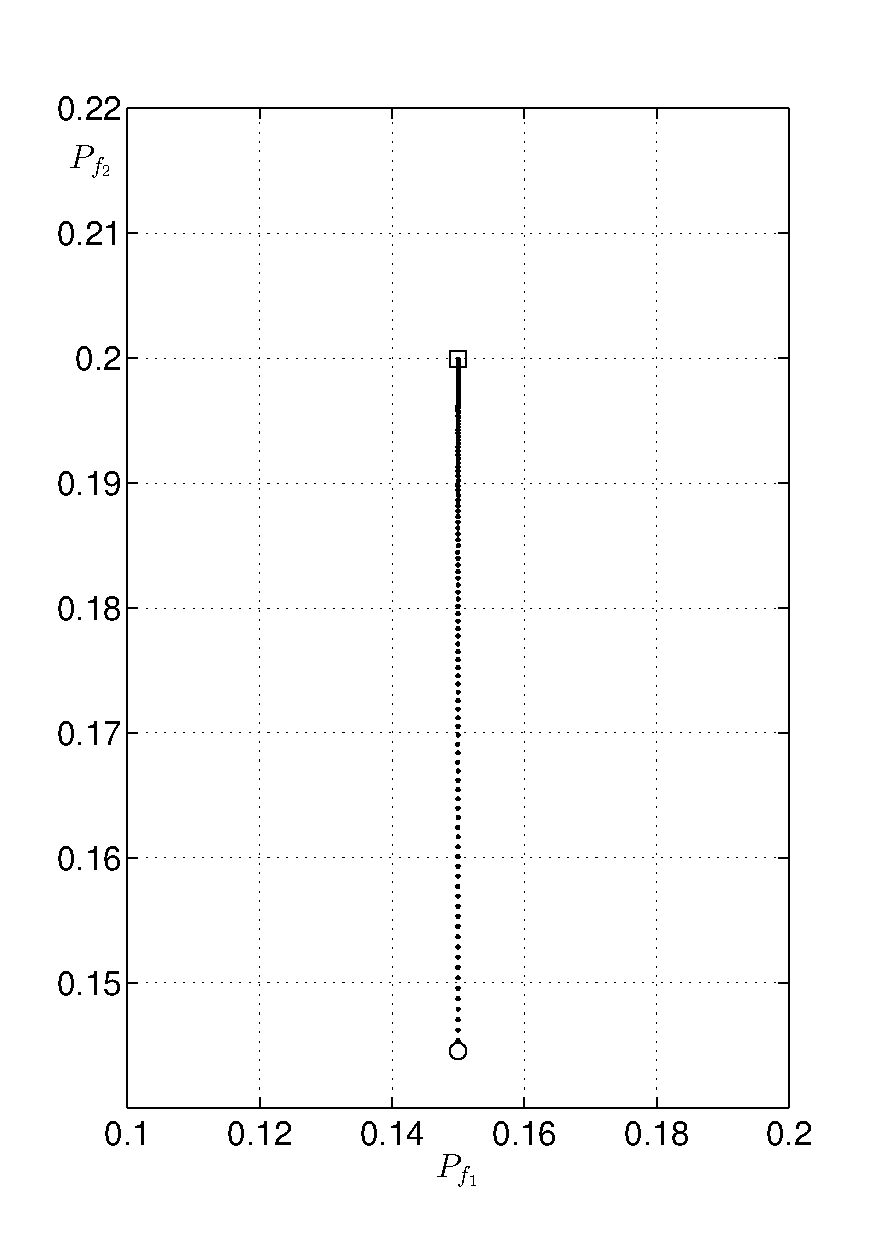
\includegraphics[width = 14cm]{2/152pf.eps}
\caption{Change of $P_{f_1}$, $P_{f_2}$ after each iteration.}
\label{fig: 2.3}
\end{figure}
\newpage
\begin{figure}[H]
\centering
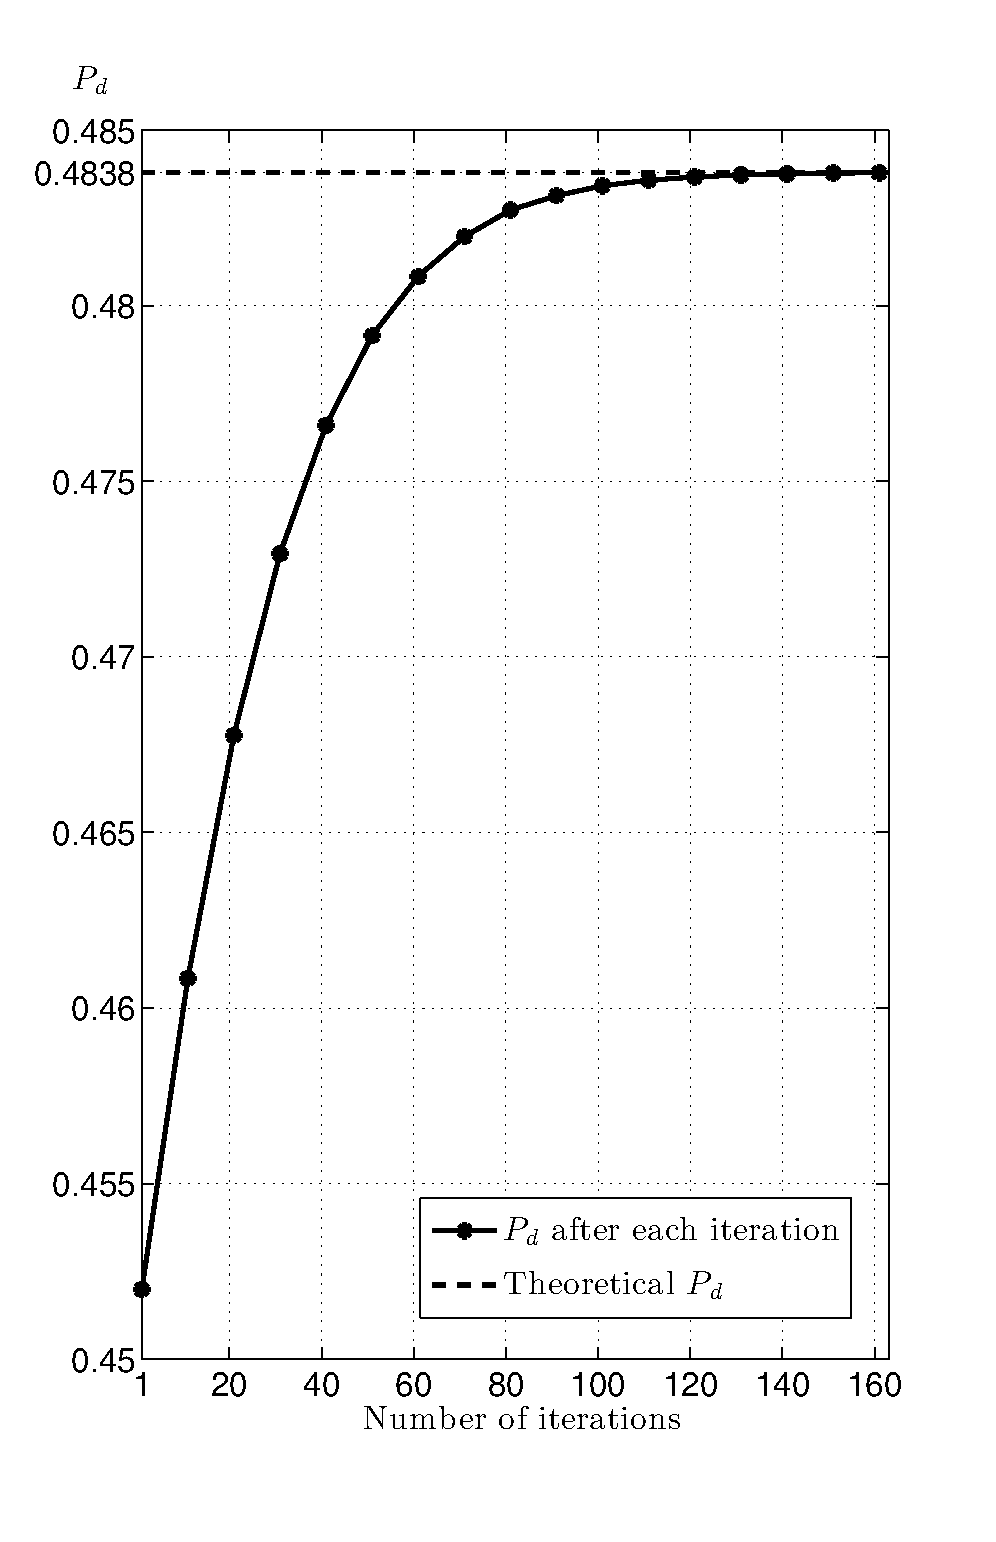
\includegraphics[width = 14cm]{2/152pd.eps}
\caption{Change of $P_d$ after each iteration.}
\label{fig: 2.2}
\end{figure}
\newpage

The weight and threshold of the final solution are

\[
\begin{split}
\omega_1 = 0.9208\\
\omega_2 = 0.0792\\
t = 1.7889
\end{split}
\]
Since $k_1 = \omega_1 t$ and $k_2 = \omega_2 t$, we can see
\[
\begin{split}
k_1 &= 1.6474\\
k_2 &= 0.1416
\end{split}
\]
The performance measure of the decision rule are
\[
\begin{split}
P_{f_1} &= 0.1500\\
P_{f_2} &= 0.1999\\
P_d &= 0.4838
\end{split}
\]


We can see, $P_{f_1}$ is equal to its associated constraint $c_1$  while $P_{f_2}$ is $0.0001$ smaller than its associated  constraint $c_2$. 


Then we consider an ENP test for $c_1 = 0.2$ and $c_2 = 0.4$.
After the initiation, the weight and threshold are $\omega_1 = \omega_2 = 0.5$, $t =2.0278$, and the corresponding performance measures are $P_{f_1}  = 0.2000$, $P_{f_2} = 0.1720$ and $P_d = 0.5367$. The algorithm carries $14$ iterations of weight  threshold adjustment. The corresponding $(P_{f_1}, P_{f_2})$ are   
marked as '*' and connected by a dotted line in Fig. \ref{fig: 2.4}. 
The $(P_{f_1}, P_{f_2})$ point of the initialization is plotted as  a 'o' and the $(P_{f_1}, P_{f_2})$ point of the final solution are plotted as a '$\square$'. The change of $P_d$ after each iteration is plotted in Figure \ref{fig: 2.5}. 
The dotted line in Figure \ref{fig: 2.5} represents the theoretical probability of detection under constraint $\mathbf{P}_f \leq \mathbf{c}$. This value is derived through the exhaustive search method approached last section.  


The weight and threshold of the final solution are
\[
\begin{split}
\omega_1 = 1.000\\
\omega_2 = 0.000\\
t = 1.4075
\end{split}
\]
Since $k_1 = \omega_1t$ and $k_2 = \omega_2t$, we can see
\[
\begin{split}
k_1 &= 1.4072\\
k_2 &= 0.000
\end{split}
\]
The performance measure of the decision rule are
\[
\begin{split}
P_{f_1} &= 0.2\\
P_{f_2} &= 0.2799\\
P_d &= 0.5629
\end{split}
\]

\begin{figure}[H]
\centering
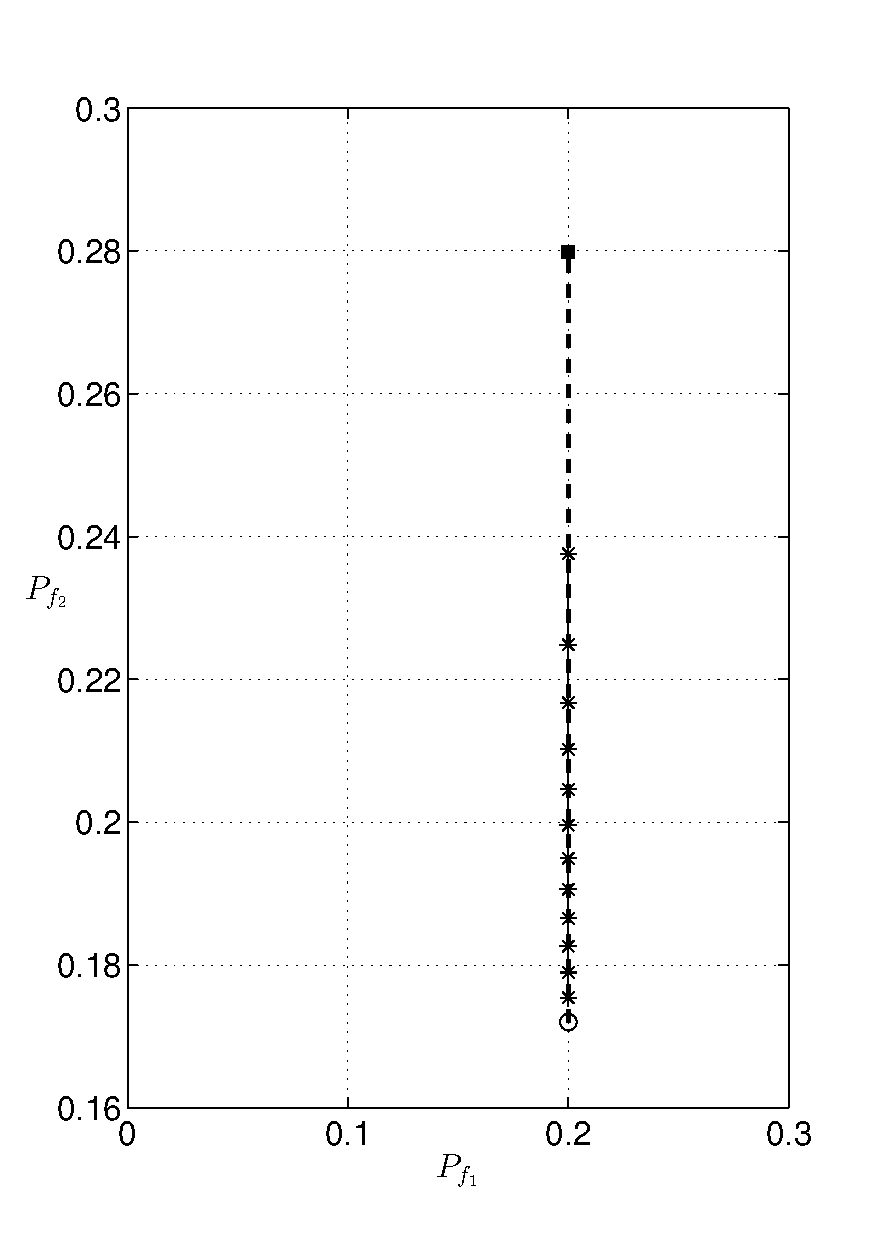
\includegraphics[width = 14cm]{2/24pf.eps}
\caption{Change of $P_{f_1}$, $P_{f_2}$ after each iteration.}
\label{fig: 2.4}
\end{figure}
\newpage
\begin{figure}[H]
\centering
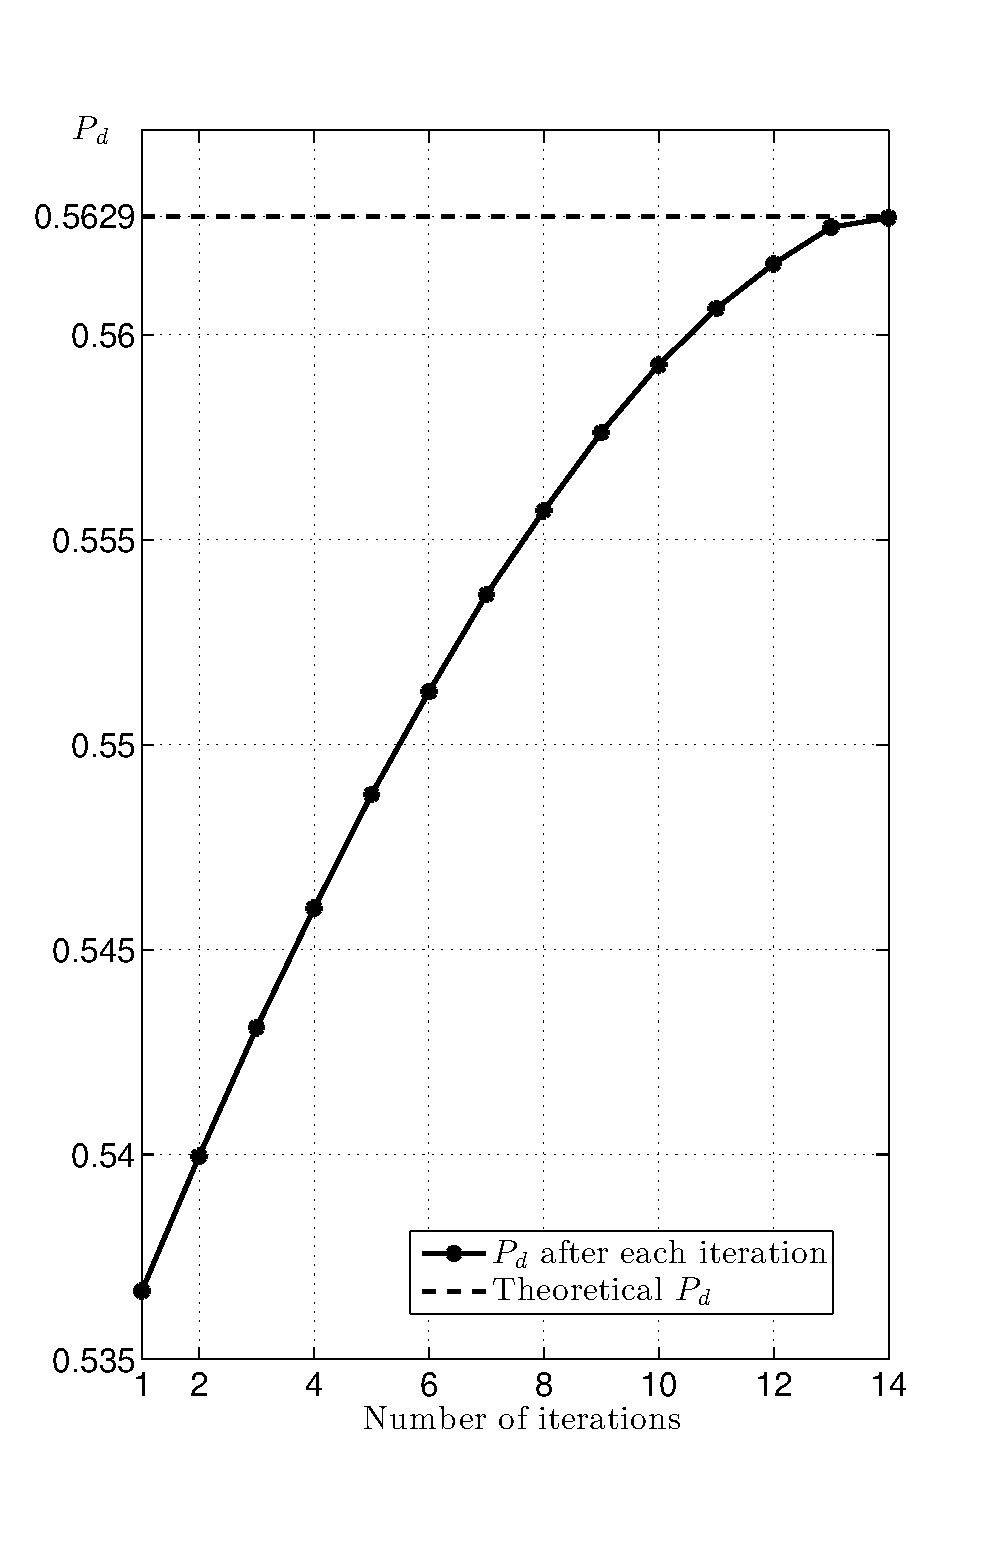
\includegraphics[width = 14cm]{2/24pd.eps}
\caption{Change of $P_d$ after each iteration.}
\label{fig: 2.5}
\end{figure}
\newpage


Thus we can observe, $P_{f_1}$ is equal to its constraint ($c_1 = 0.2$) while $P_{f_2}$ is much smaller than its constraint ($c_2 =0.4$). However since $\omega_2$ is equal to zero, $P_{f_2}$ does not have to be close to $c_2$ to stop the algorithm. By using the exhaustive search method approached last section, we can verify the largest probability of detection under the constraint $\mathbf{P}_f \leq \mathbf{c}$ is $0.5629$, which is equal to the solution generated by the algorithm.
